\section*{Diagnóstico de sesgo y varianza}
En pos de entender cómo se comportan el sesgo y la varianza en nuestros modelos, realizamos mediciones para
construir curvas de complejidad y aprendizaje para tres de nuestros mejores modelos: KNN, SVM y Árboles de Decisión.

\subsection*{Curvas de Complejidad}
Usando nuestros mejores modelos obtenidos durante la exploración de hiperparámetros, graficamos el desarrollo del error
a partir de cambiar ciertos hiperparámetros de cada modelo. Observemos a continuación cómo quedaron los gráficos:

\begin{figure}[H]
    \centering

    \subfloat[\centering Curva de complejidad para Árboles \label{fig:comp1}]{
        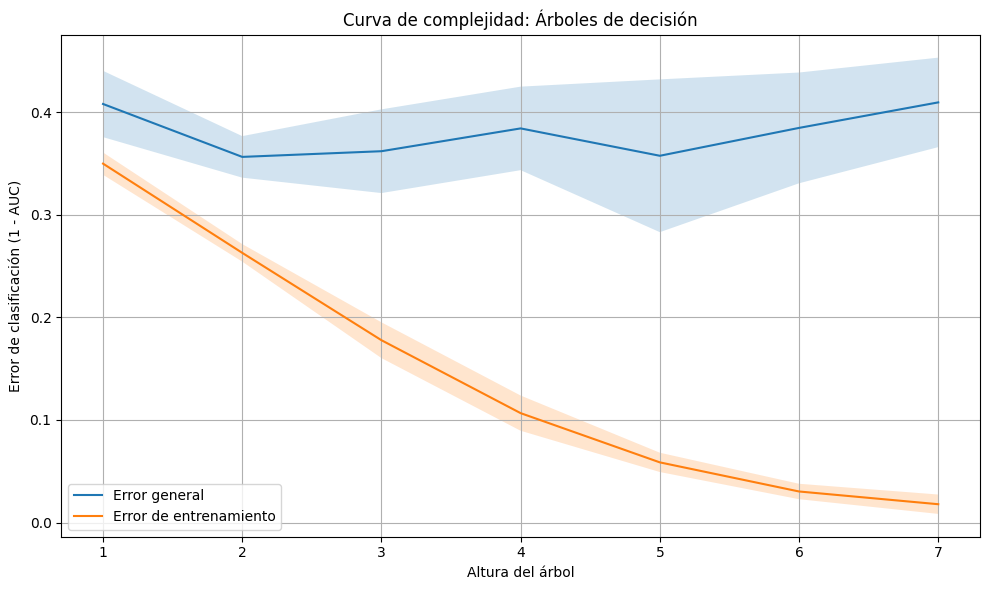
\includegraphics[width=0.5\linewidth]{img/complejidad_arbol.png}
    }
    \subfloat[\centering Curva de complejidad para SVM \label{fig:comp3}]{
        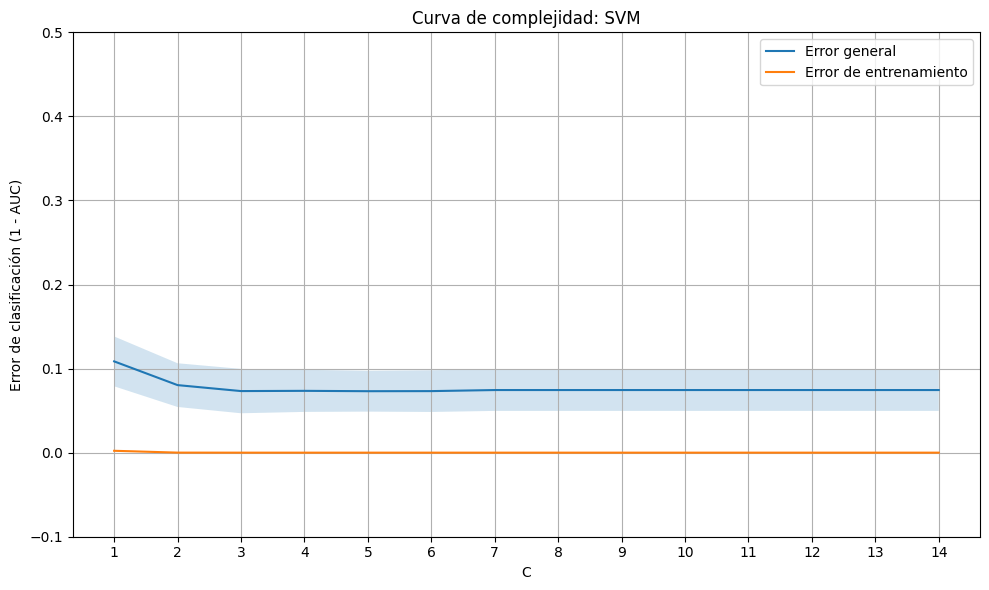
\includegraphics[width=0.5\linewidth]{img/complejidad_svm.png}
    }
 
    \vspace{0.1cm}

    \subfloat[\centering Curva de complejidad para KNN \label{fig:comp2}]{
        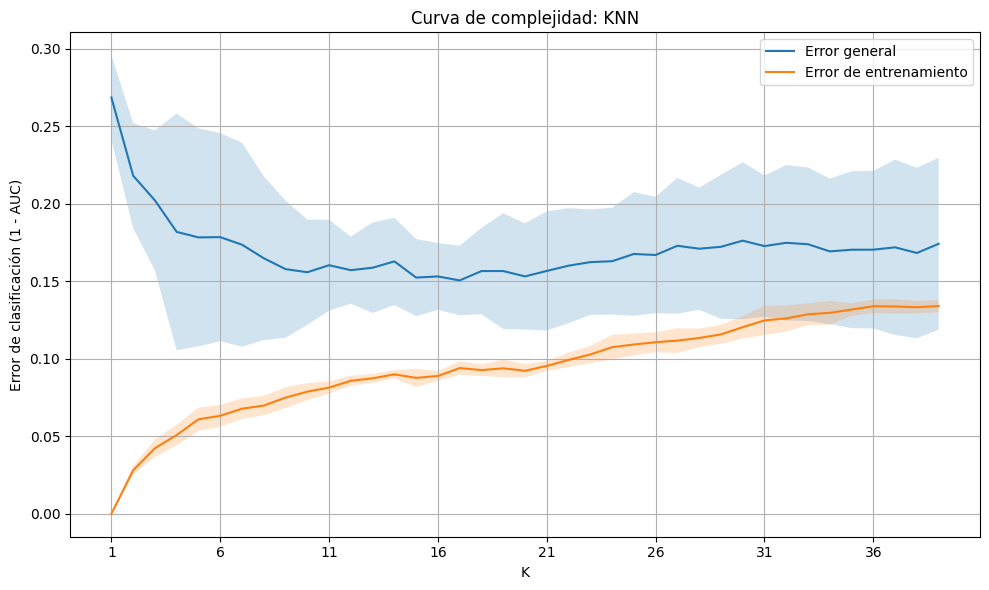
\includegraphics[width=0.5\linewidth]{img/complejidad_knn.png}
    }
    \label{fig:distr}
\end{figure}

Las curvas muestran el error, el cual computamos como 1 - \textit{AUC-ROC} en funcion del hiperparámetro explorado, donde 
el error general es a partir de la predicción del fold que no usó para entrenar, y el error de entrenamiento surge de predecir los mismos datos
utilizados para entrenar el modelo.

En \ref{fig:comp1}, podemos ver que para el \textbf{Decision Tree} calculamos el error con distintos valores de la altura desde 1 a 10, ya que explorar valores mas altos no aporta
más ganancia en este dataset.

A medida que aumenta la altura del árbol, el sesgo disminuye significativamente, dejando el error de entrenamiento en 0. Sin 
embargo, el error general no baja a medida que aumenta la altura del árbol, aumentndo la varianza y mostrando que el modelo está 
overfitteando. Por otro lado, en las alturas más bajas del árbol se ve un error de entrenamiento muy alto, mostrando que, en estas
circunstancias, el modelo subajusta. La altura óptima para este modelo sería entre 2 y 5, ya que hay un buen \textit{trade-off} entre
el sesgo y la varianza.

Observando \ref{fig:comp3}, podemos notar que el modelo de \textbf{Support Vector Machines} comienza teniendo un error general alto y un error de entrenamiento muy bajo,
indicando alto sesgo. Sin embargo, al agrandar \texttt{C}, el error general baja entre hasta \texttt{C} = 1 y \texttt{C} = 3, y luego se mantiene constante; mientras que el error
de entrenamiento se mantiene bajo, por lo que el sesgo baja significativamente, y la varianza se mantiene en valores bajos.
Esto indica que este modelo SVM ya tiene suficiente flexibilidad para separar bien las clases y añadir capacidad extra (agrandando el valor de \texttt{C}) no empeora la generalización.

En cuanto a \textbf{K-Nearest Neighbors}, en \ref{fig:comp2} se observa un comportamiento contrario al de los árboles. Valores bajos de \texttt{K} llevan a modelos que sobreajustan. Al subir este hiperparámetro, 
el modelo comienza a subajustar. Con \texttt{K} bajos, el modelo se acopla perfectamente a los datos de entrenamiento,
produciendo bajo sesgo y alta varianza. Con \texttt{K} entre 7 y 15, se observan los valores óptimos de  \textit{trade-off} entre sesgo y varianza,
y, al llegar a los valores más altos de \texttt{K}, se reduce notablemente la varianza, con una suba considerable de el sesgo.


\subsection*{Curvas de Aprendizaje}
Para los mismos modelos, también graficamos curvas de aprendizaje. Hicimos uso de la función de de la biblioteca scikitlearn llamada \texttt{learning\_curve}. Como parámetro de cuántas instancias contemplar en el conjunto de entrenamiento, usamos un array de 5 valores equitativamente espaciados entre 0.1 y 1.0, que representa la proporción de instancias utilizadas en cada ejecución. Al hacer 5-fold cross validation para armar las curvas, terminamos entrenando con 34, 110, 187, 263 y 340 instancias a la vez.

\begin{figure}[H]
    \centering

    \subfloat[\centering Curva de aprendizaje para árboles de decisión \label{fig:apr1}]{
        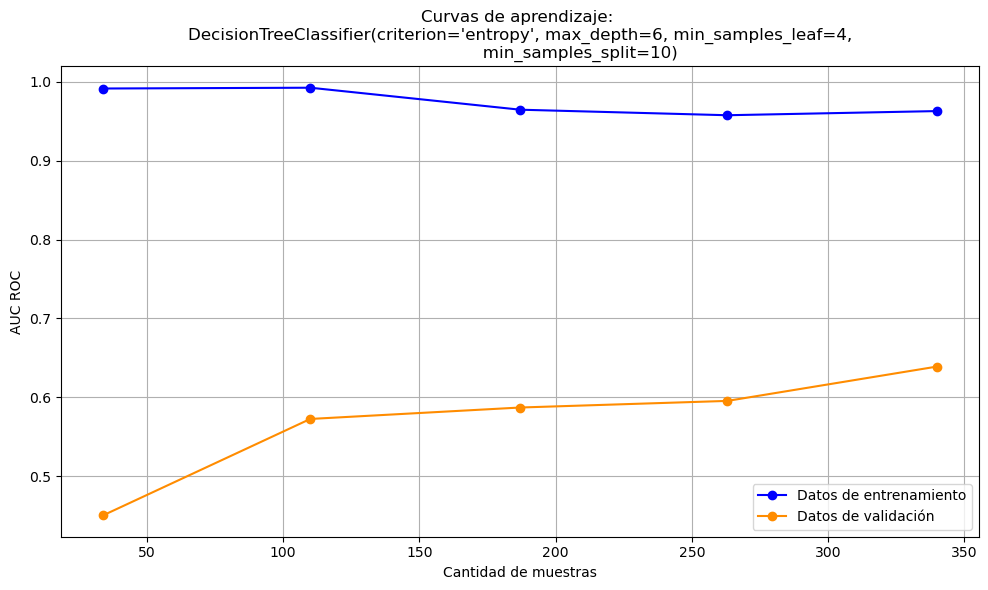
\includegraphics[width=0.45\linewidth]{img/aprendizaje_arbol.png}
    }
    \subfloat[\centering Curva de complejidad para SVM \label{fig:apr3}]{
        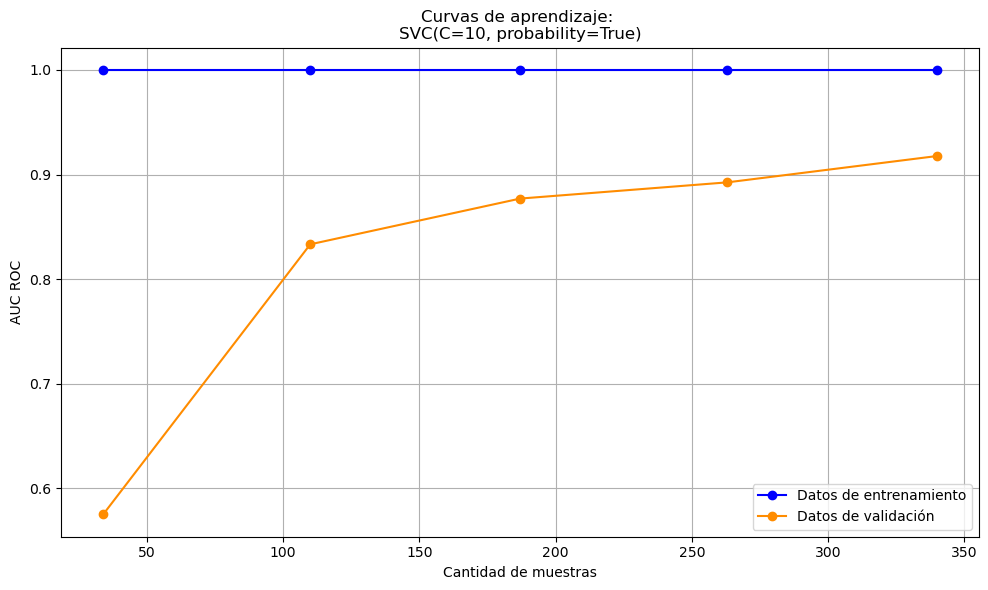
\includegraphics[width=0.45\linewidth]{img/aprendizaje_svm.png}
    }

    \vspace{0.3cm}

    \subfloat[\centering Curva de aprendizaje para KNN \label{fig:apr2}]{
        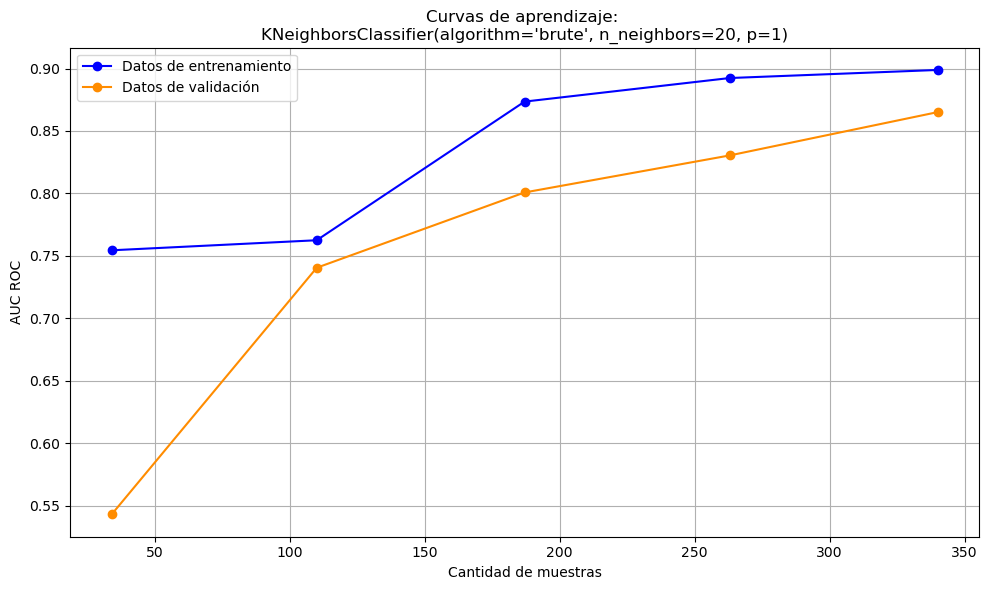
\includegraphics[width=0.45\linewidth]{img/aprendizaje_knn.png}
    }
    \subfloat[\centering Curva de aprendizaje para LDA \label{fig:apr4}]{
        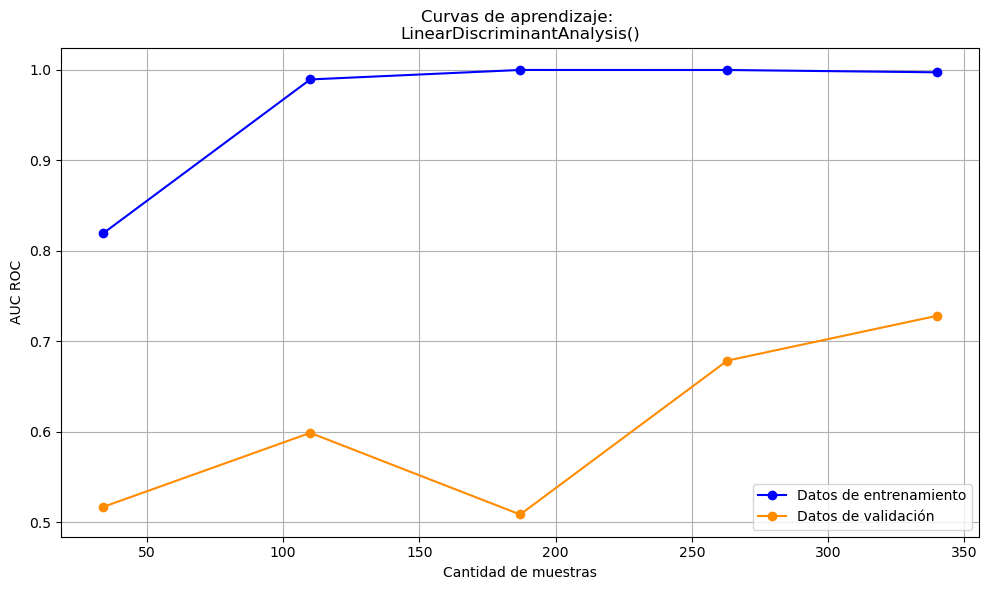
\includegraphics[width=0.45\linewidth]{img/aprendizaje_lda.png}
    }

    \caption{Curvas de complejidad para distintos modelos}
    \label{fig:distr}
\end{figure}

Para \textbf{árboles de decisión}, en la figura \ref{fig:apr1}, con las primeras proporciones de instancias de entrenamiento (34 y 110 instancias), el modelo parece estar sobreajustando. Vemos que en entrenamiento tiene un AUC-ROC tendiente a 1, pero en los datos de evaluación el AUC-ROC está por debajo o apenas supera AUC-ROC de 0.5 que tendría un clasificador dummy. Pero a medida que incrementa la proporción de datos utilizados para entrenar, también incrementa el AUC-ROC de validación y disminuye el de entrenamiento, achicando la brecha entre estos. Podemos asumir que con una proporción baja de datos de entrenamiento el modelo no lograba captar patrones subyacentes a los datos, aprendiendo características que le permitían ajustar a los datos que conocía pero que no eran representativos del dataset en general.

En cuanto a \textbf{Support Vector Machines}, en la figura \ref{fig:apr3} se puede ver que la performance en evaluación medida con AUC-ROC sube muchísimo al aumentar la cantidad de muestras, principalmente entre 1 y 110. Luego de las 100 muestras, el modelo sigue mostrando mejoras en su comportamiento, pero con incrementos más suaves. Sin embargo, más allá de que el puntaje en evaluación mejora, la performance sobre los datos de entrenamiento se mantiene en 1 sin importar la cantidad de muestras que se usen para entrenar, lo cuál puede indicar un sobreajuste cuando se cuenta con bajas cantidades de datos.

Para \textbf{K-Nearest Neighbors}, podemos interpretar la figura \ref{fig:apr2} en base al hiperparámetro de \texttt{n\_neighbors}, que en nuestro mejor modelo es 20. Esto es un número bastante elevado en comparación a con cuántas instancias entrenamos en las primeras iteraciones. No es sorpresivo que con 20 vecinos, usando 34 instancias, el AUC-ROC de entrenamiento sea relativamente bajo y el de evaluación ($\approx 0.55$) sea similar al AUC-ROC del clasificador que predice la clase más frecuente; ya que estamos seleccionando \texttt{n\_neighbors} $\approx$ cantidad de instancias. Al incrementar la cantidad de instancias vistas, podemos ver que todos los puntajes AUC-ROC aumentan proporcionalmente, tanto los de entrenamiento como los de validación.


Y por último, con \textbf{Linear Discriminant Analysis}, en la figura \ref{fig:apr4} la performance en entrenamiento aumenta a medida que subimos la cantidad de muestras hasta 187, y luego se mantiene constante. Sin embargo, cuando observamos el AUC-ROC con datos de validación, el gráfico presenta más variaciones, alcanzando el mínimo cuando se entrena con 187 muestras. Esto puede sugerir que en esa iteración el modelo sobreajusta sobre los datos de entrenamiento, y no logra generalizar correctamente para nuevas instancias. Podría estar relacionado a qué instancias en particular fueron agregadas a la muestra en esa iteración. Sería posible que ese conjunto de 187 muestras no sea representativo de la distribución del conjunto de los datos, impidiendo aprender características útiles para generalizar. Luego de alcanzar el mínimo, si seguimos aumentando la cantidad de instancias la performance en validación sí mejora significativamente.


\subsection*{Exploración de Random Forest}
Para este experimento, construimos un modelo Random Forest con 200 árboles. La idea fue explorar el hiperparámetro \texttt{max\_features}, que limita cuántos atributos se pueden considerar cada vez que se busca el mejor corte para el árbol. Los valores considerados fueron  1, $log_2(\#atributos)$, 10, $sqrt(\#atributos)$, 50, 100, 200 (es decir, $\#atributos$).
 \begin{figure}[H]
    \centering

    \subfloat[\centering Curvas de complejidad variando el hiperparámetro \texttt{max\_features} \label{fig:rf1}]{
        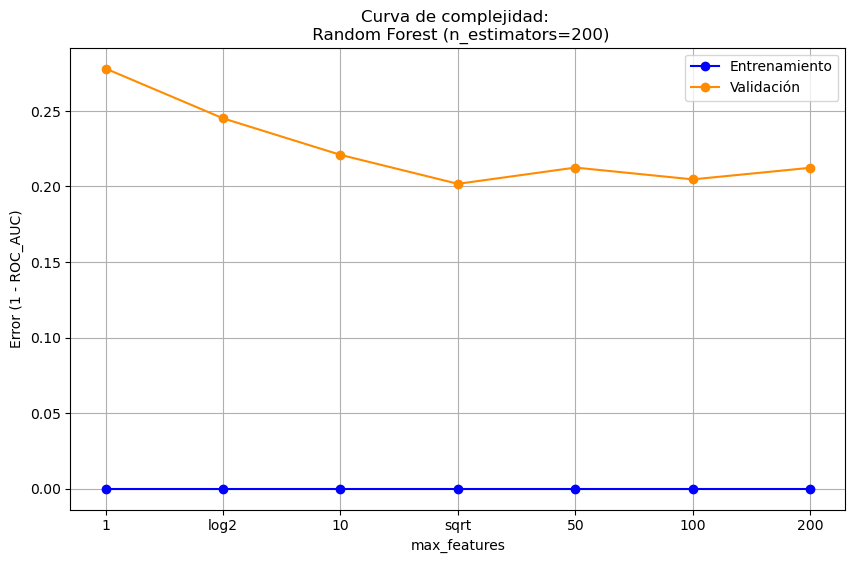
\includegraphics[width=0.45\linewidth]{img/rf1.png}
    }
    \subfloat[\centering Curvas de aprendizaje utilizando \texttt{max\_features} = $sqrt(\#atributos)$ \label{fig:rf2}]{
        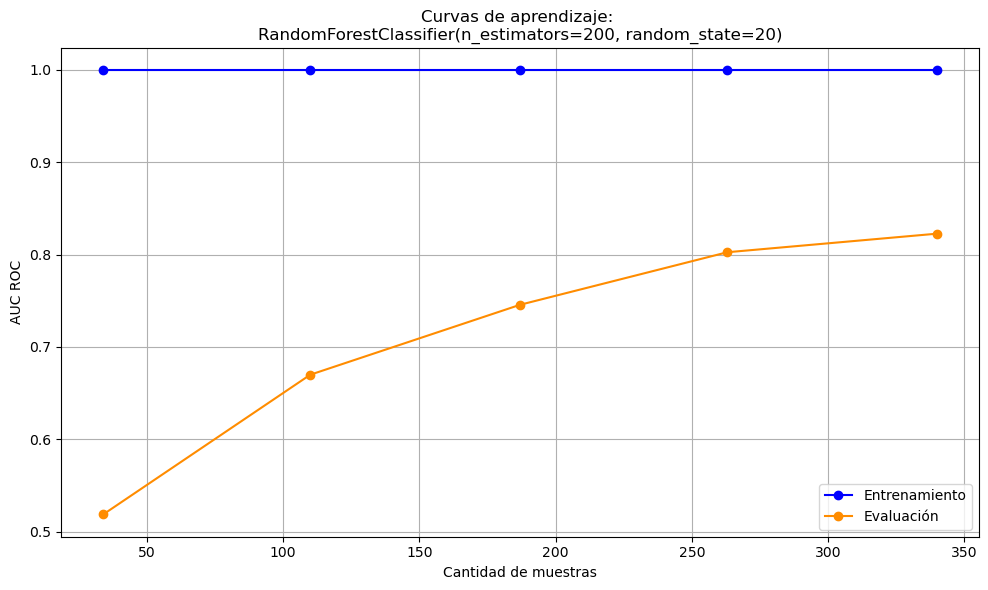
\includegraphics[width=0.45\linewidth]{img/rf2.png}
    }
    \caption{Resultados de experimentos con Random Forest}
    \label{fig:distr}
\end{figure}

En la figura \ref{fig:rf1} generamos curvas de complejidad para cada uno de los modelos resultantes, en base a estos valores de \texttt{max\_features}. Con los datos de entrenamiento, cualquier cantidad de atributos genera un árbol que ajusta perfectamente. La diferencia se ve en los datos no vistos en entrenamiento. Podemos observar que el error en validación es mínimo utilizando $sqrt(\#atributos) \approx 14$. También que se llega al mayor error con los valores más bajos: con 1, $log_2 \approx 8$ y 10. Es decir, elegiríamos no limitar más que $sqrt(\#atributos)$ la cantidad de atributos máxima a contemplar en los cortes. Contemplar menos atributos parece limitar la capacidad de generalización del modelo.

Utilizando el mínimo valor observado, \texttt{max\_features} $= sqrt(\#atributos)$, graficamos también una curva de aprendizaje, que se puede visualizar en la figura \ref{fig:rf2}. Podemos ver una evolución considerable en la performance con datos de validación. A medida que aumentamos la cantidad de datos, también sube la performance, llegando hasta AUC-ROC de $\approx  0.83$. Sin embargo, más allá de que la curva sube, se observa que el aumento de performance no es constante, y tiende a estancarse, por lo que agregar más datos no debería presentar un aumento significativo. Por otro lado, la performance en entrenamiento se mantiene constante sin importar la cantidad de muestras utilizadas, presentando un AUC-ROC de 1 tomando tanto la mínima cantidad de muestras como la máxima. A partir de esto, podríamos estar ante un sobreajuste cuando tenemos baja cantidad de instancias, y, a medida que aumentan, el modelo comienza a generalizar mejor.
